\subsubsection{Programmflussdiagramm}
\label{subsubsec:Programmflussdiagramm}

\paragraph{Bootloader-Section}\mbox{}
In Abbildung \ref{fig:Programmfluss_Atmega2560} wird der Programmfluss der Atmega2560-Software aufgezeigt. Bei einschalten des Mikrocontrollers wird in der Bootloader-Section zuerst der Bootloader gestartet (Boot Loader Flash Section). Sofern keine neue Software über die UART0-Schnittstelle kommt, so beginnt das cocktailspezifische Programm (Application Flash Section). Sofern eine neue Software über die UART0-Schnittstelle gesendet wird, wird die kommende Software in diese Application Flash Section geschrieben und das Programm nach der Übertragung gestartet.

\paragraph{Init-Section}\mbox{}
Wird das Programm gestartet, beginnt die Init-Section. Hier werden die zuerst die Main-Variabeln initialisiert. Danach werden die Adressen der Funktionen ins Programm geladen mittels den h-Files. Die Interfaces (SPI, Uart, I/O's) müssen als erstes initialisiert werden, damit die Initialisierung der SPI-Devices stattfinden kann und Boot-Informationen über eine gewünschte Schnittstelle angezeigt werden können (z.B Uart0 ==> Computer). Sobald die Schnittstellen initialisiert wurden, werden die Devices initialisiert. Dazu gehören die SD-Karte, der FOC-Treiber und der Gate-Treiber. Daraufhin werden die Speicher-Strukturen initialisiert, welche für die User-Applikation (Tabelle \ref{fig:Softwareuebersicht_Atmega2560} in Kapitel \ref{subsec:Strukturplan_Atmega}) gebraucht werden. Die Struktur und Anwendung der Speicherplätze wird in Kapitel \ref{subsec:Dynamic_Linked_Lists} erklärt. Zu guter Letzt wird die Startanzeige des Displays geladen.

\paragraph{Main-Loop}

Da die Maschine nur auf Inputs reagieren muss, werden im Main-Loop nur die Buffer der Devices abgefragt. Sobald ein Terminator-Zeichen ankommt (z.B ein carriage return \\r der UART0-Schnitstelle oder 0xFF 0xFF 0xFF der UART1-Schnittstelle), werden die zuvor empfangenen Daten interpretiert und verarbeitet.
\newpage

\begin{figure}[h!]
	\centering
	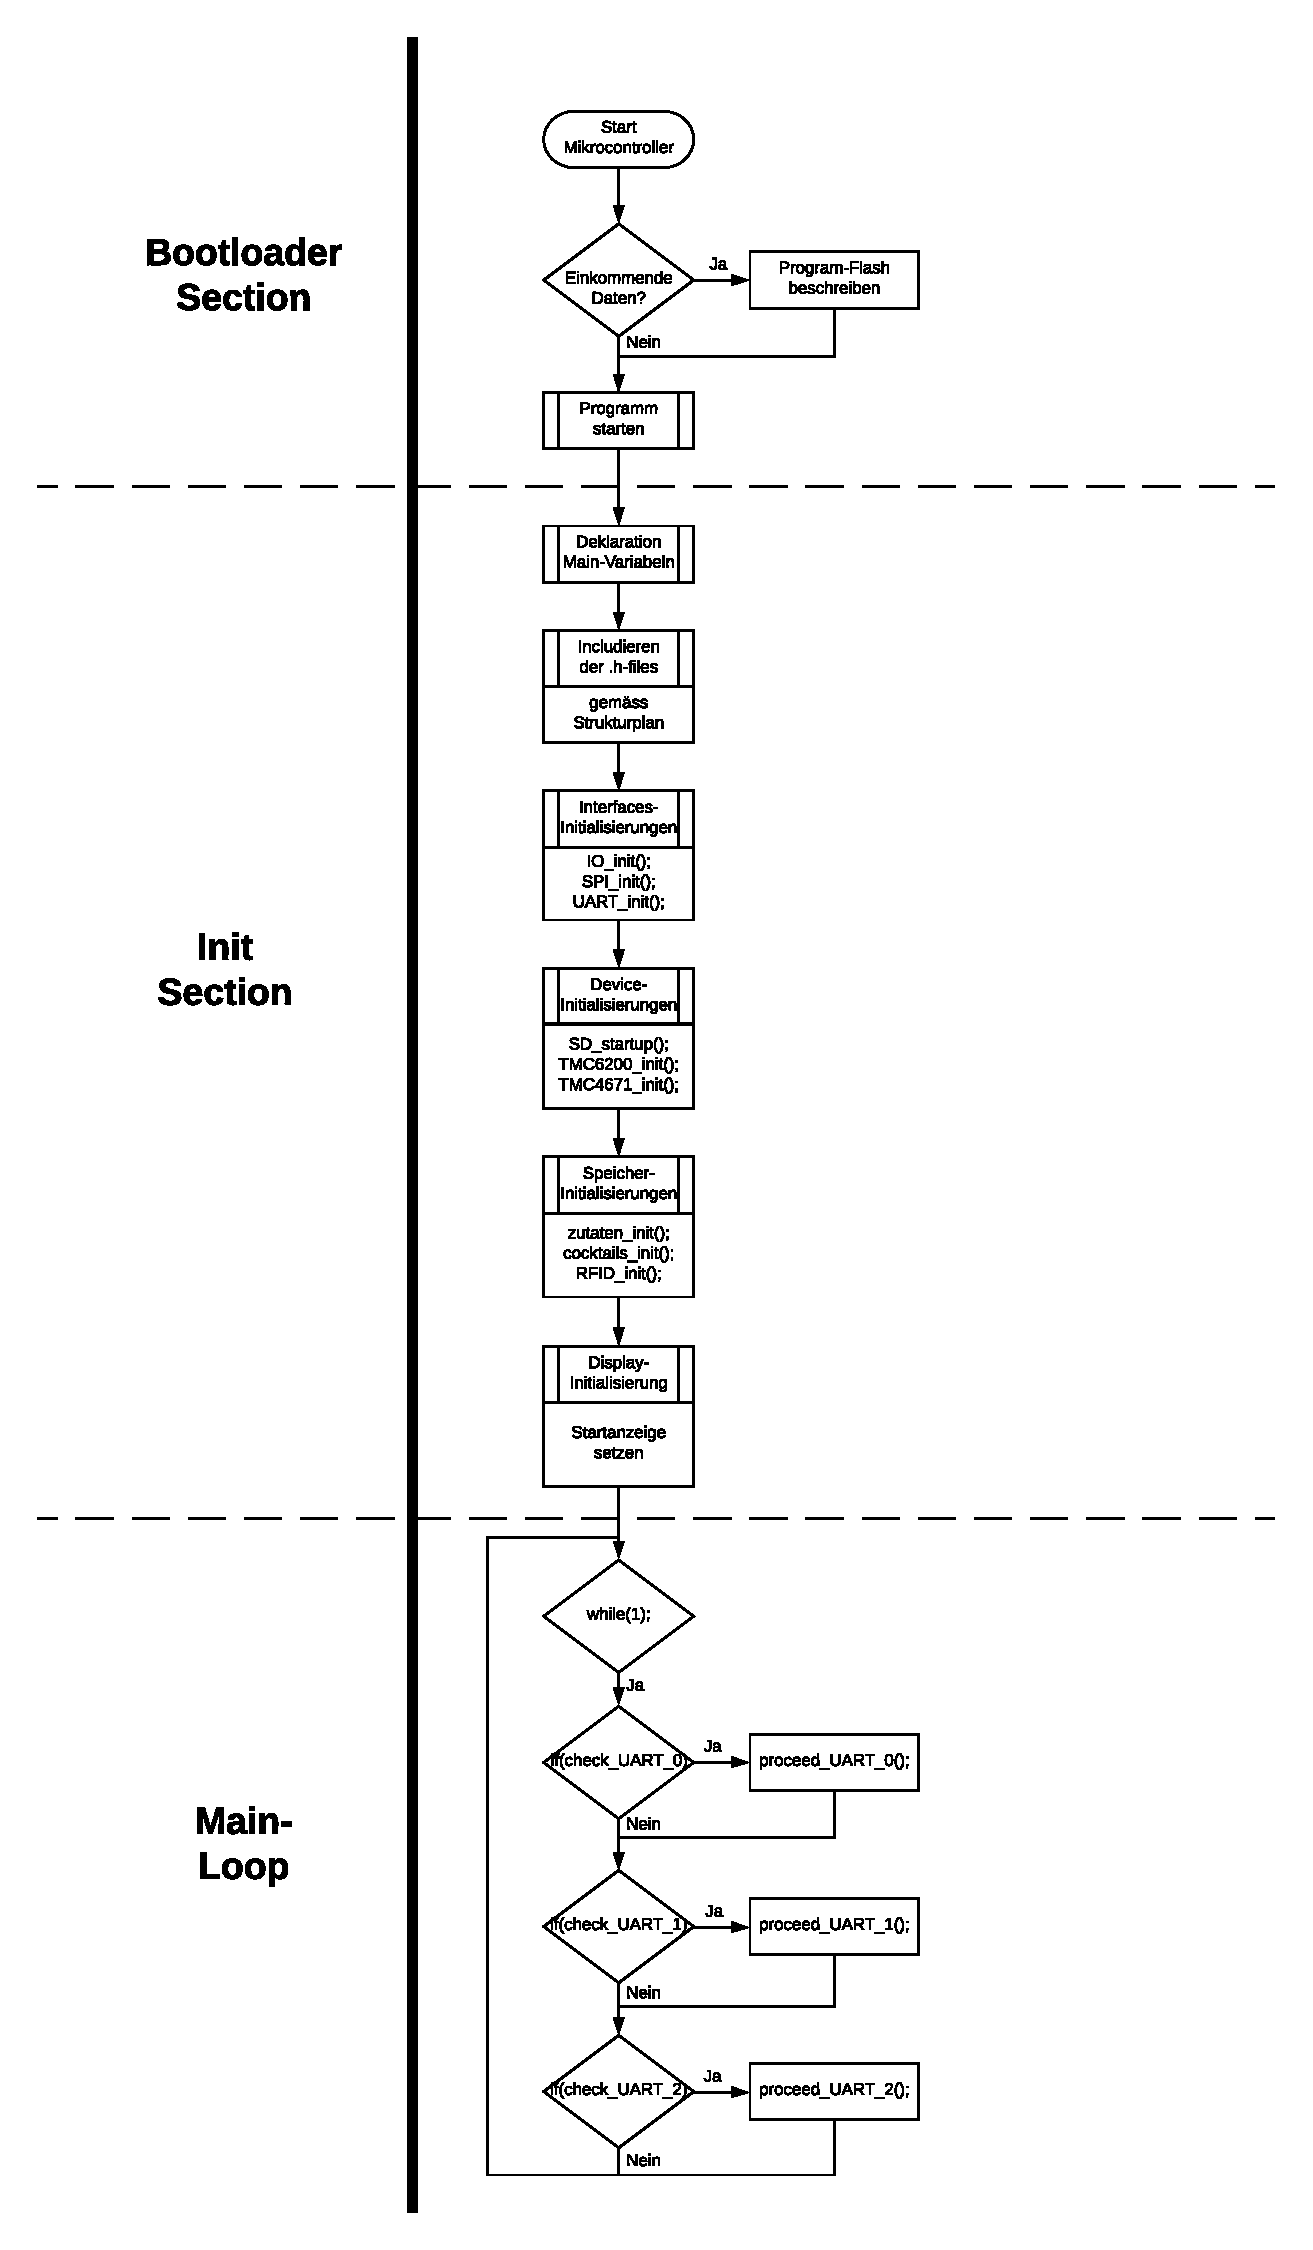
\includegraphics[width=0.5\textwidth]{graphics/Programmfluss_Atmega2560.pdf}
	\caption{Programflussdiagramm Atmega2560.}
	\label{fig:Programmfluss_Atmega2560}
\end{figure}
\newpage


\subsubsection{Doubly Dynamic Linked Lists Allgemein}

Eine Doppelt verkettete Liste ist eine gängige Datenstruktur, welche verwendet wird, sobald es in der Anwendung wichtig ist, in einer Liste hoch und runter zu bewegen und effizient und ohne grossen Aufwand sogenannte Nodes\footnote{Nodes = Knoten} hinzugefügt werden müssen. Im Folgenden wird von Elementen statt Nodes gesprochen. Die Idee dabei ist, dass für jedes Element zwei Pointer zu initialisieren, welche auf das nächste oder vorhergehende Element zeigen. Nebst den Zeigern auf die umliegenden Elemente enthält das Element die gewünschten Daten. Um zu wissen, ob das Ende oder der Beginn erreicht wurde, werden zwei zusätzliche Zeiger initialisiert, welche auf das erste und/oder letzte Element zeigen (Head und Tail). Um zu wissen, auf welches Element zurzeit gezeigt wird, gibt es einen Zeiger auf dieses Element (actual).

\todo{cite Text: https://perlgeek.de/de/artikel/doppelt-verkettete-listen}

Abbildung \ref{fig:Doubly_Linked_List_2_00} zeigt eine Grundsätzliche Struktur der beschriebenen Liste mit head, tail und Elementen.

\begin{figure}[h!]
	\centering
	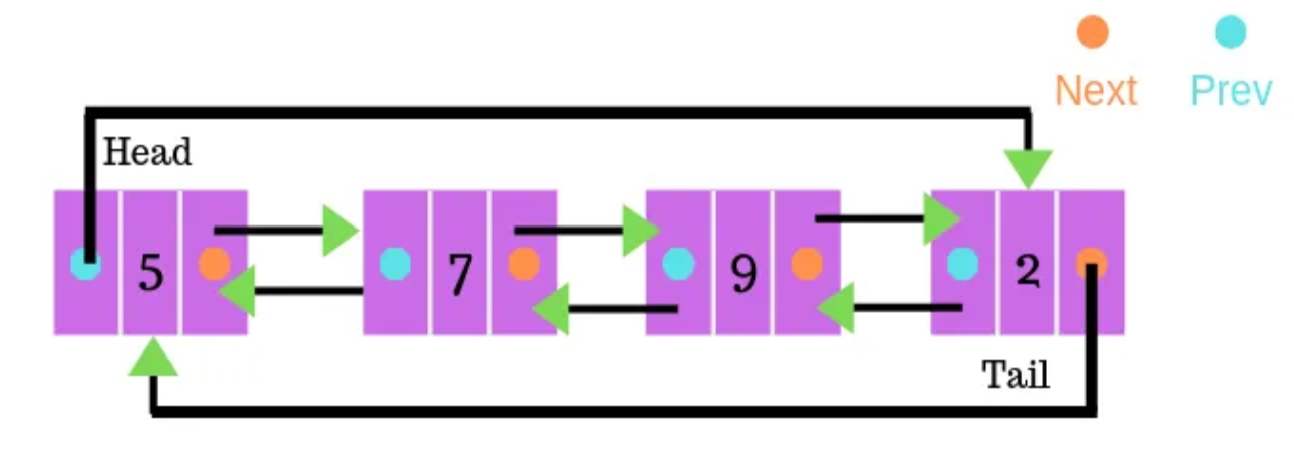
\includegraphics[width=0.5\textwidth]{graphics/Doubly_Linked_List_2_00}
	\caption{Doppelt verkettete Liste mit zwei Elementen.}
	\label{fig:Doubly_Linked_List_2_00}
\end{figure}

\todo{cite Bild: https://learnersbucket.com/tutorials/data-structures/circular-doubly-linked-list-in-javascript/}

In Abbildung \ref{fig:Doubly_Linked_List_2_0} wird nur der start-Pointer (head) initialisiert, ohne auf ein Element zu zeigen (NULL). Sobald der benötigte Speicherplatz des Elementes alloziiert wurde, wird der Zeiger auf die angelegte Struktur (Element) gelegt. Dem Head-Zeiger wurde nun ein Element zugewiesen und der Beginn der Liste wurde definiert.

\begin{figure}[h!]
	\centering
	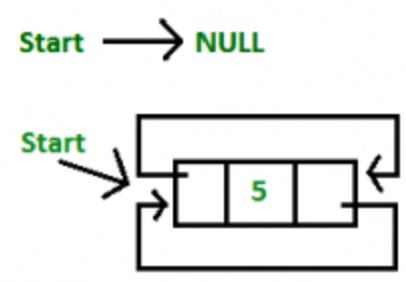
\includegraphics[width=0.5\textwidth]{graphics/Doubly_Linked_List_2_0}
	\caption{Doppelt verkettete Liste mit zwei Elementen.}
	\label{fig:Doubly_Linked_List_2_0}
\end{figure}

\todo{cite Bild:https://www.geeksforgeeks.org/doubly-circular-linked-list-set-1-introduction-and-insertion/}

Abbildung \ref{fig:Doubly_Linked_List_2_1} zeigt eine bestehende Liste mit zwei Elementen. Ein drittes Element soll am Schluss eingefügt werden. Dazu muss zuerst der Speicherplatz für das neue Element alloziiert werden (Data, next, prev). Danach können die Zeiger der bestehenden Elemente (in diesem Falle noch head und tail) umgelegt werden und die Zeiger des neuen Elementes auf das vorhergehende und nächste Element gelegt werden. Auch der tail-Zeiger muss nun auf das neue Element gelegt werden.

\begin{figure}[h!]
	\centering
	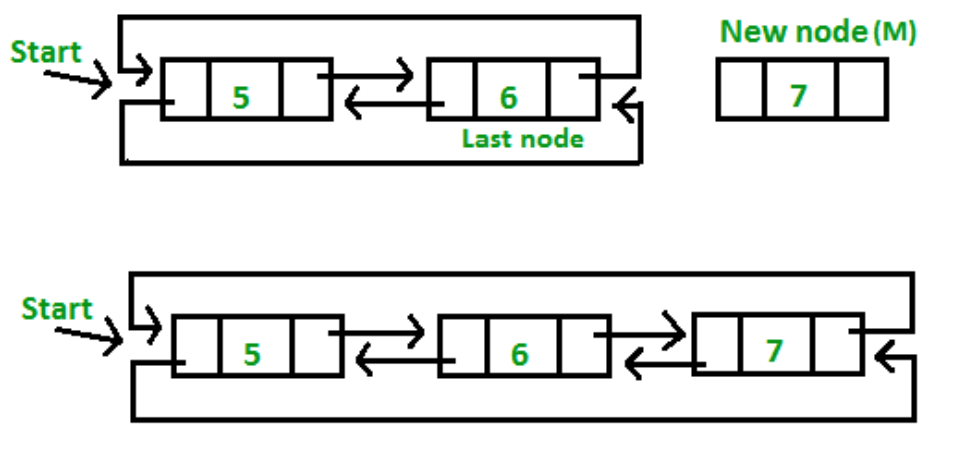
\includegraphics[width=0.5\textwidth]{graphics/Doubly_Linked_List_2_1}
	\caption{Doppelt verkettete Liste mit zwei Elementen.}
	\label{fig:Doubly_Linked_List_2_1}
\end{figure}

\todo{cite Bild:https://www.geeksforgeeks.org/doubly-circular-linked-list-set-1-introduction-and-insertion/}

Abbildung \ref{fig:Doubly_Linked_List_2_2} zeigt ebenfalls eine bestehende Liste mit zwei Elementen. Ein drittes Element soll am Beginn eingefügt werden. Dazu muss zuerst der Speicherplatz für das neue Element alloziiert werden (Data, next, prev). Danach können die Zeiger der bestehenden Elemente (in diesem Falle noch head und tail) umgelegt werden und die Zeiger des neuen Elementes auf das vorhergehende und nächste Element gelegt werden. Auch der head-Zeiger muss nun auf das neue Element gelegt werden.

\begin{figure}[h!]
	\centering
	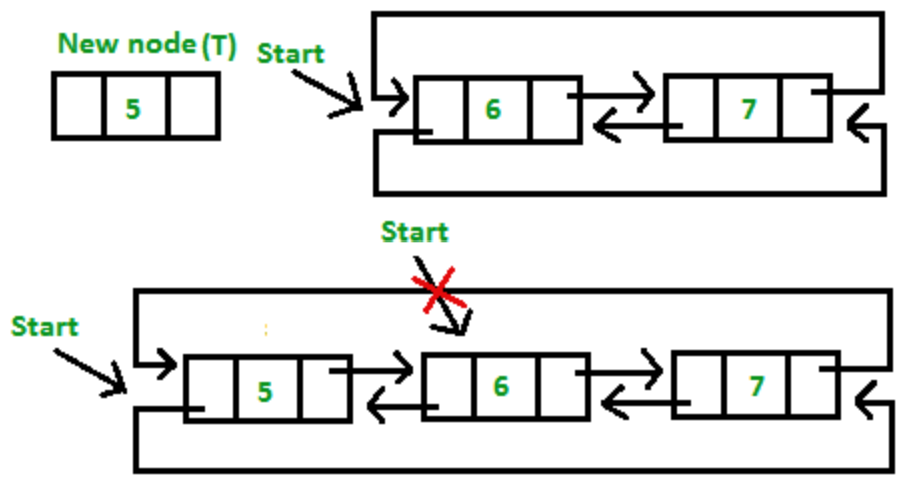
\includegraphics[width=0.5\textwidth]{graphics/Doubly_Linked_List_2_2}
	\caption{Doppelt verkettete Liste mit zwei Elementen.}
	\label{fig:Doubly_Linked_List_2_2}
\end{figure}

\todo{cite Bild:https://www.geeksforgeeks.org/doubly-circular-linked-list-set-1-introduction-and-insertion/}

Abbildung \ref{fig:Doubly_Linked_List_2_3} zeigt eine bestehende Liste mit vier Elementen. Ein fünftes Element soll in der Mitte eingefügt werden. Dazu muss zuerst der Speicherplatz für das neue Element alloziiert werden (Data, next, prev). Danach können die Zeiger der bestehenden Elemente umgelegt werden und die Zeiger des neuen Elementes auf das vorhergehende und nächste Element gelegt werden.

\begin{figure}[h!]
	\centering
	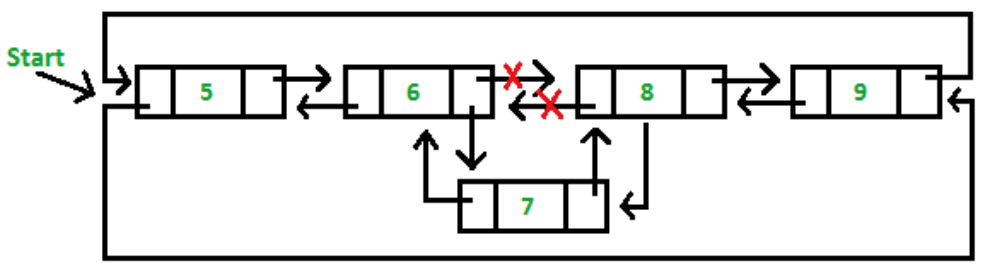
\includegraphics[width=0.5\textwidth]{graphics/Doubly_Linked_List_2_3}
	\caption{Doppelt verkettete Liste mit zwei Elementen.}
	\label{fig:Doubly_Linked_List_2_3}
\end{figure}

\todo{cite Bild:https://www.geeksforgeeks.org/doubly-circular-linked-list-set-1-introduction-and-insertion/}

\subsubsection{Doubly Dynamic Linked Lists Cocktailmixer}

Im Falle des Cocktailmixers werden verschiedene Listen verwendet. Dazu gehören die folgenden Elemente:

\begin{itemize}
\item Cocktail-Liste (Files)
\item Zutaten-Liste (Files)
\item Tag-Liste (Maschine)
\item Zutaten-in-Maschine-Liste (Maschine)
\end{itemize}

Die Cocktail- und die Zutaten-Liste beinhalten nur die Nummer des Files, welches sich auf der SD-Karte befindet. Wird ein Cocktail oder eine Zutat benötigt, so werden die Daten temporär von der SD-Karte in einen Struct im Programmspeicher geladen. Dies wird gemacht, da während der Entwicklung der Programmspeicher mit zu vielen Daten gefüllt wurde, was zur Folge hatte, dass der Mikrocontroller abstürzte. Im Vergleich zum kompletten Cocktail, welcher ca. 80 Bytes Speicher braucht, benötigt das File nur eines. Ein einziger Struct, welcher immer neu geladen wird, reicht aus, um die benötigten Informationen zu extrahieren und verwenden. Jeder Cocktail und jede Zutat wird separat auf der SD-Karte gespeichert.

Die Tag-Liste sowie die Liste der Zutaten in der Maschine werden komplett in den Programmspeicher geladen. Die beiden Listen werden bei einer Veränderung als Backup jeweils in einem File gespeichert, damit diese bei einem Neustart der Maschine wieder in den Programmspeicher geladen werden können.